\section{Classical Algorithms}\label{sec:classical-algorithms}
\localtableofcontents
\subsection{Interpolation}\label{subsec:interpolation}

Suppose that \(H_k\) is linear spatial\anote{lsi} and time invariant.
%
Suppose further that \(A_k\) is affine.
%
Then \(H \coloneqq H_k\) commutes with \(A_k\) \cite{meladcommute} and eqn.~\eqref{eqn:commuteimagingmodel} becomes
\begin{equation}
    \label{eqn:commuteimagingmodel}
    \begin{split}
        \Xk &= (D \circ A_k \circ H) (Y) + \varepsilon \\
        &= (D \circ A_k) (H(Y)) + \varepsilon \\
        &= (D \circ A_k) (V) + \varepsilon
    \end{split}
\end{equation}
%
where \(V \coloneqq H(Y)\).
%
This naturally suggests interpolation in order to recover \(V\) (since \(\Xk\), in this framing, are simply shifted samples of \(V\)).
%
Note in this context we use interpolation very broadly, i.e.,to connote filling in missing values using neighboring (in some sense --- not necessarily geometrically) values.
%
\begin{figure}
    \centering
    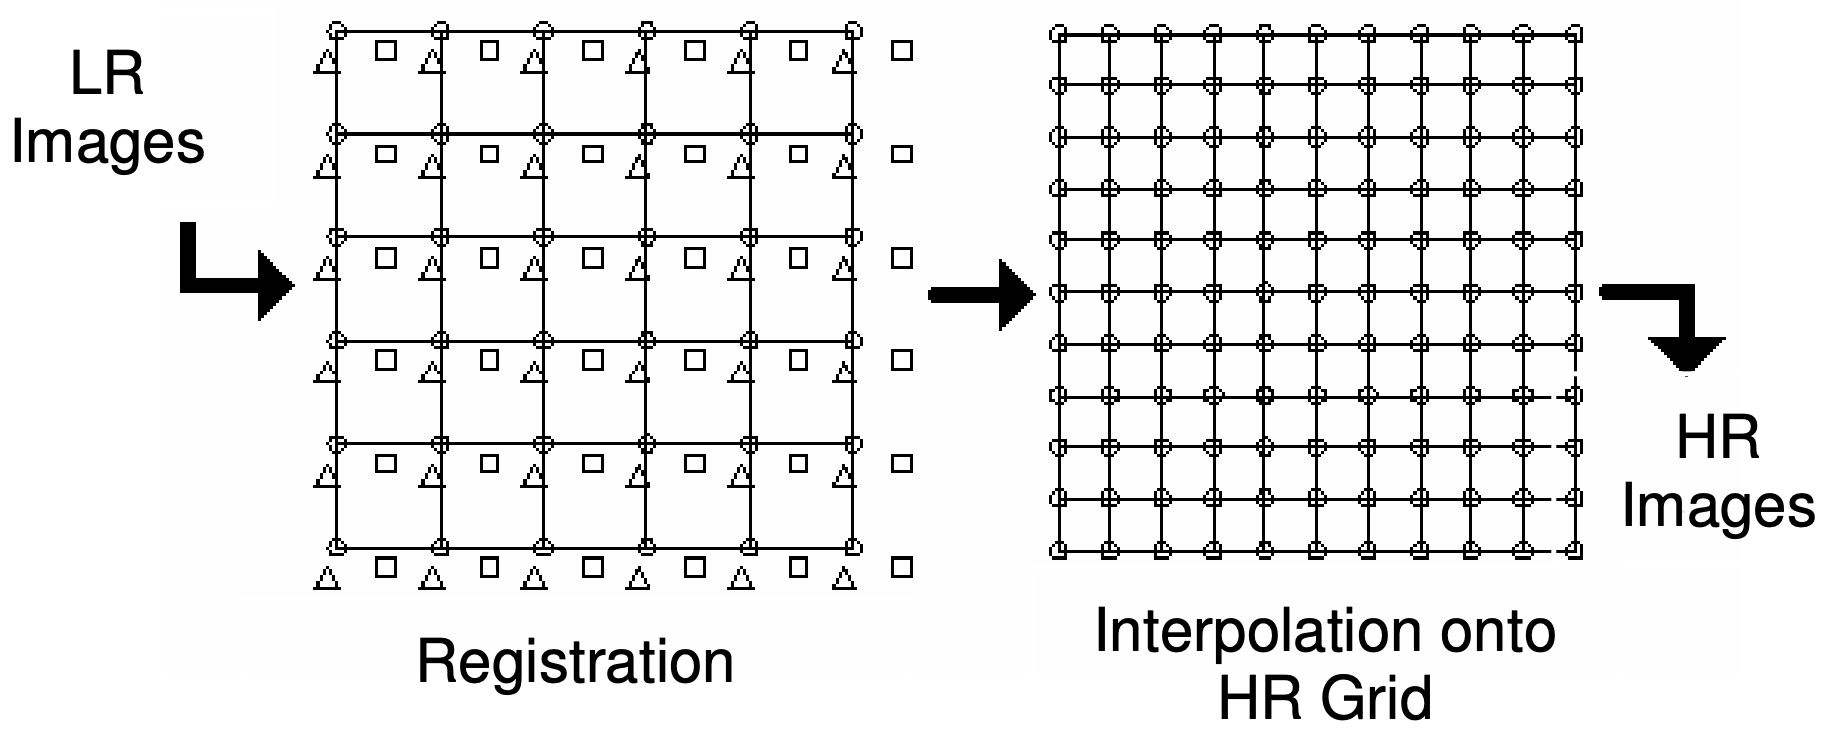
\includegraphics[width=\linewidth,keepaspectratio]{figures/classical/hrgrid.png}
    \caption{LR image registration on an HR grid \cite{Lin}.}
    \label{fig:hrgrid}
\end{figure}
This class of techniques proceed by first registering images on a high resolution grid (see figure~\ref{fig:hrgrid}) then interpolating at the missing pixels in the HR grid to recover \(V\), and finally denoising and deconvolution (of \(H\)) to recover \(Y\).
%
Since in general consecutive \(\Xk\) have non-uniform shifts (relative to \(X_1\)) the interpolation is non-uniform and improvisations on this theme use various weighting schemes for adjacent LR pixels\anote{lrpixel}.

For example Alam \text{et al.} \cite{Alam2000} uses weighted nearest neighbors: for every pixel to be interpolated the three nearest pixels are weighted inversely by their distance (according to HR grid distance) and then their weighted sum is assigned to that pixel.
%
This non-uniform interpolation is then followed by application of a Wiener filter whose design is informed by the OTF of the particular imaging system they study (which they do not estimate i.e.,they assume they can model accurately).
%
\subsubsection{Delaunay Triangulation}

\begin{figure}
    \centering
    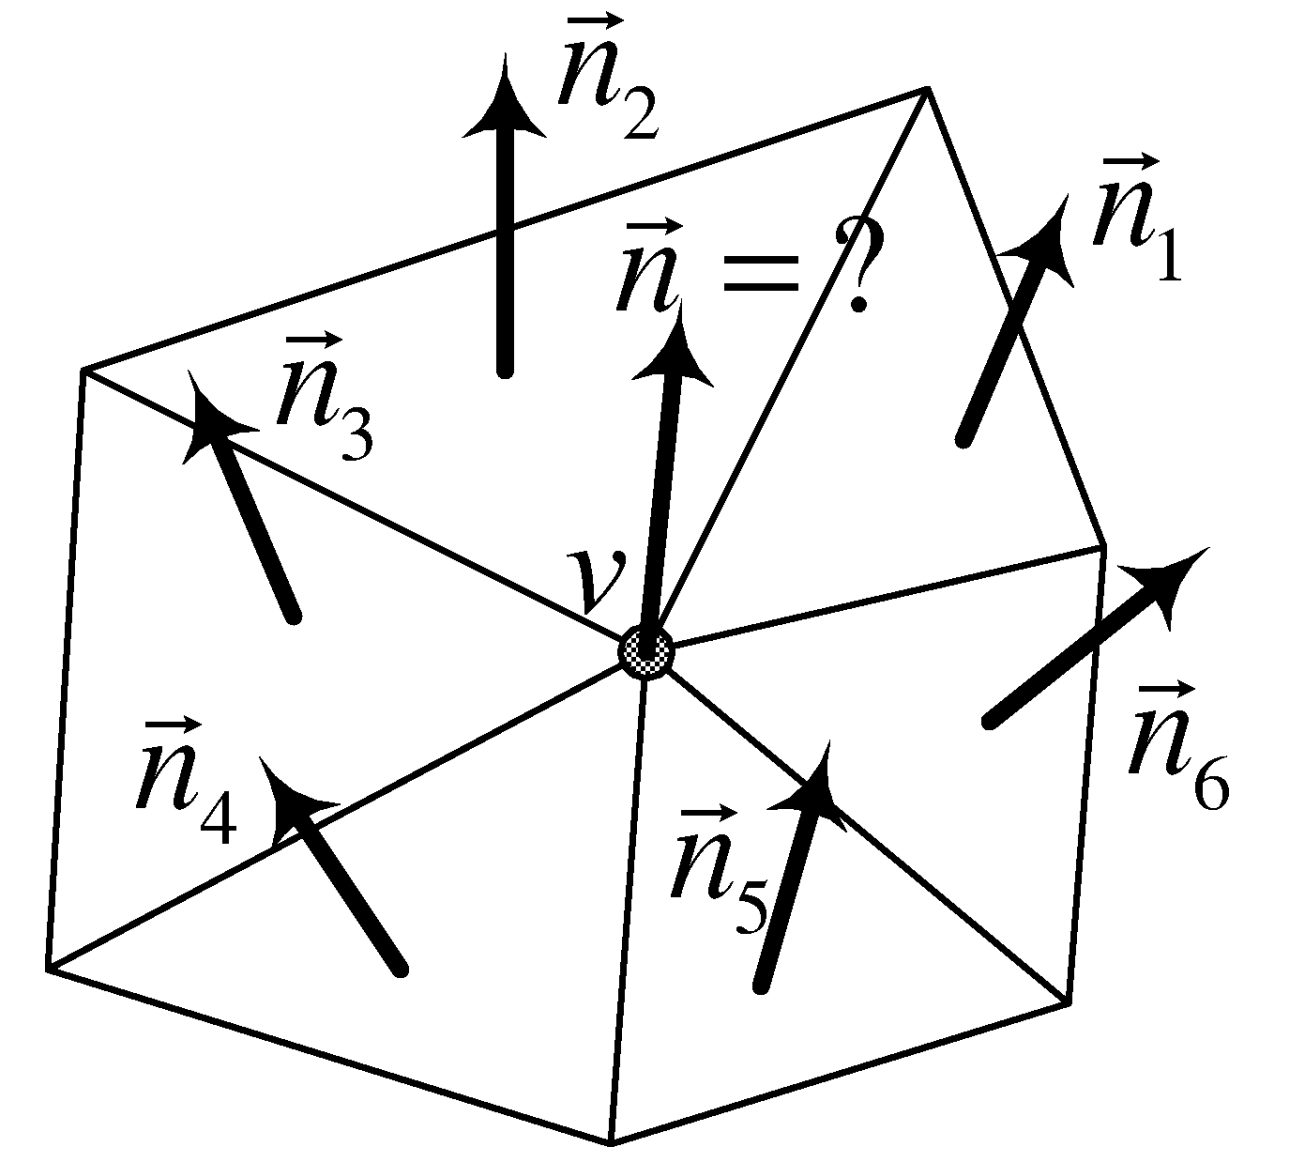
\includegraphics[width=.7\linewidth]{figures/classical/delauney.png}
    \caption{Delaunay triangulation for fitting splines at LR pixels \cite{Lertrattanapanich}. \(v\) is an LR pixel. Note that \(v\) is at \(z\) equal to the pixel value.}
    \label{fig:delauney}
\end{figure}
Lertrattanapanich \text{et al.} \cite{Lertrattanapanich} base their algorithm on interpolants which require knowledge of gradients (e.g. splines) and mediate the non-uniform sampling by using a weighted average (by area) of those gradients in adjacent Delaunay cells; to be precise they produce a Delaunay triangulation of all LR pixels and compute the gradients (see figure~\ref{fig:delauney}) according to
\begin{align*}
    \vec{n} = \sum_{i=1}^m \frac{B_j \vec{n_j}}{B}   & \text{ where } B=\sum_{i=1}^m B_i                              \\
    \frac{\partial z}{\partial x} = -\frac{n_x}{n_z} & \text{ and }  \frac{\partial z}{\partial y} = -\frac{n_y}{n_z}
\end{align*}
where \(B_i\) is the area of the \(i\)th Delaunay cell.
%
Unfortunately this intricate solution is not robust to noise in real images.
\subsubsection{Wiener Filter}
A more sophisticated method for non-uniform interpolation uses parametric models for the auto-correlation between LR pixels and the cross-correlation between LR pixels and interpolated pixels to estimate wiener filter weights \cite{wiener}.
%
These weights are then used to average nearby pixel values.
%
The algorithm operates on a sliding \textit{estimation window} whose dimensions \(D_x, D_y\) are chosen such that the effective sampling rate exceeds the Nyquist rate for a given \(\rho_c\).
\begin{figure}
    \centering
    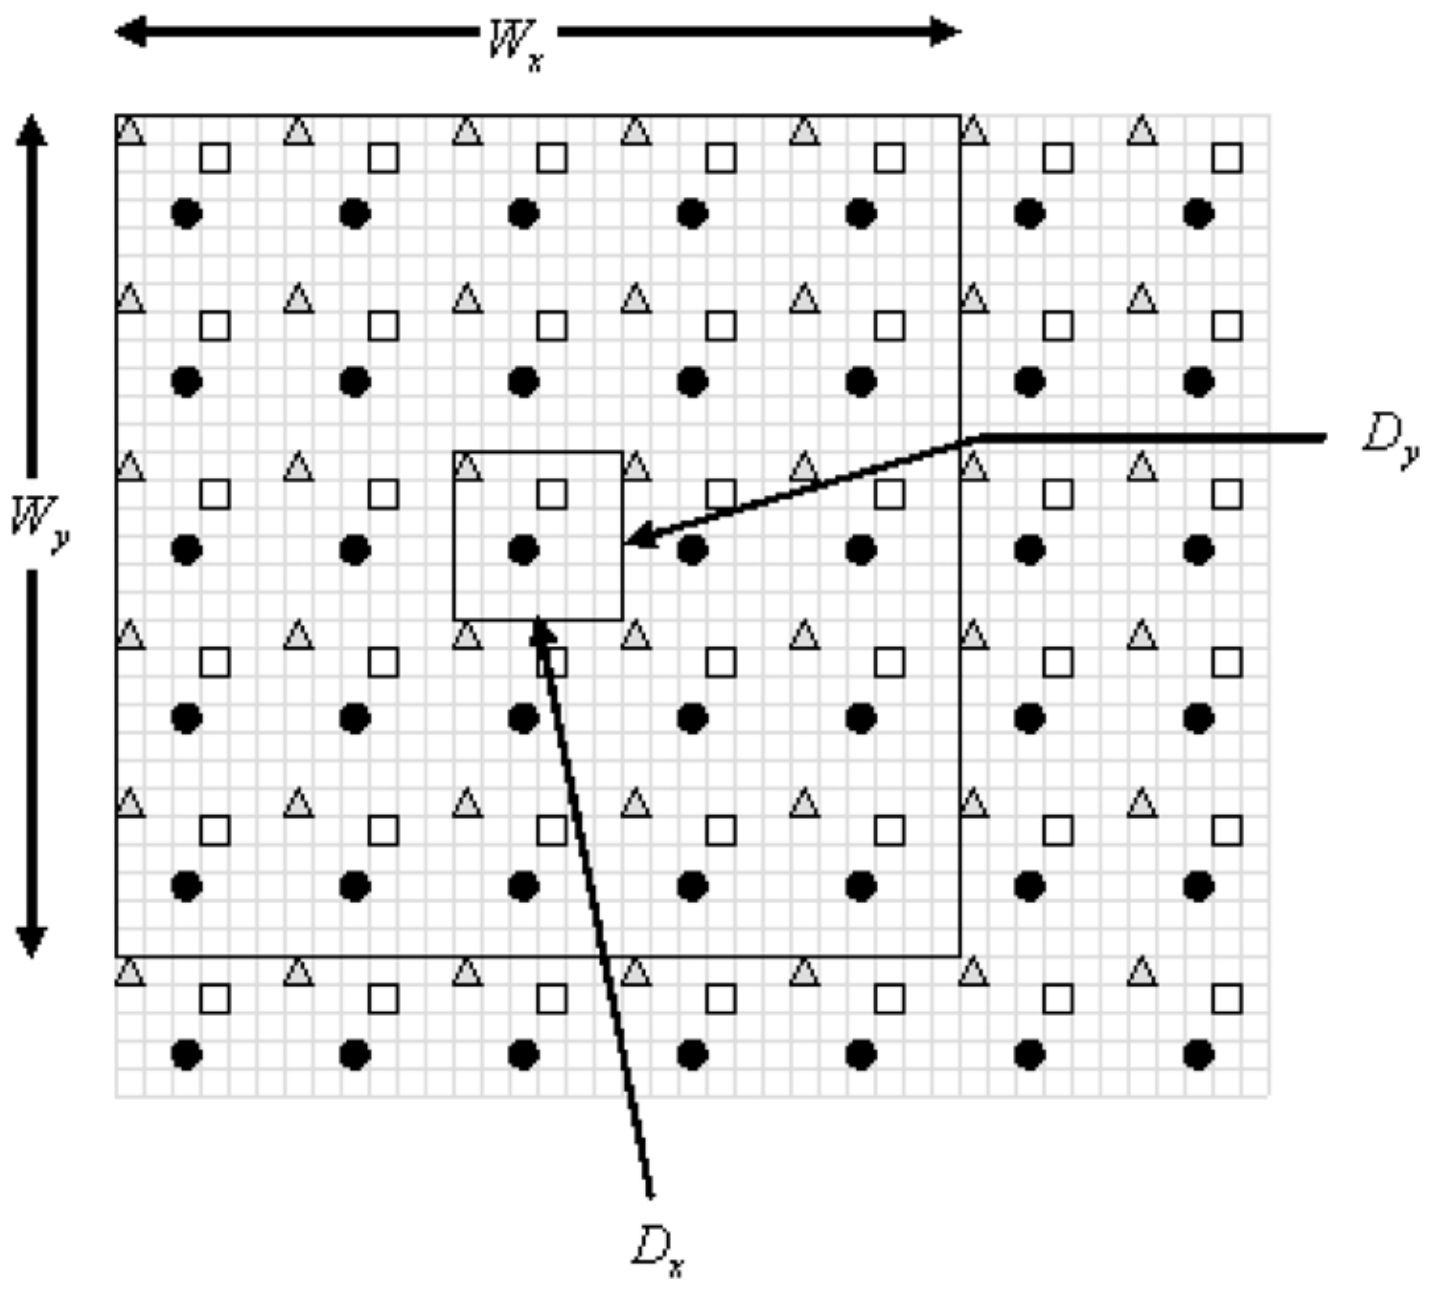
\includegraphics[width=.7\linewidth]{figures/classical/wiener.png}
    \caption{Wiener filter super resolution estimation window of dimension \(D_x \times D_y\) and observation window of dimension \(W_x \times W_y\) \cite{wiener}.}
    \label{fig:wiener}
\end{figure}
The pixel values for the estimation window are a function of the wiener filter weights of nearby LR pixels within an \textit{observation window} whose dimensions \(W_x, W_y\) are an integer multiple of \(D_x, D_y\) (see figure~\ref{fig:wiener}).
%
The weights \(\bm{w}\) are defined as the solution to the minimum mean squared error (MMSE) filter problem, i.e.,the finite impulse response (FIR) wiener filter:
\begin{equation}
    \bm{w} = R^{-1}\bm{p}
\end{equation}
where \(R\) is the auto-correlation of the LR pixels in the observation window and \(\bm{p}\) is the cross-correlation between the pixels to be estimated and the LR pixels.
%
Then \(R\) and \(\bm{p}\) are both constructed by sampling a parametric model that weights pixels in the observation window according to distance:
%
\(R\) is constructed by sampling from
\begin{equation}
    C_1(r) \coloneqq \sigma_{d}^2 \rho^{r} \ast G(r)
\end{equation}
and \(\bm{p}\) is constructed by sampling from
\begin{equation}
    C_2(r) \coloneqq \sigma_d^2 \rho^{r} \ast G(r) \ast G(-r)
\end{equation}
In the case of \(R\), \(r\) is distance on the HR grid, \(\sigma_d\) is related to the empirical variance of all LR pixels in a given observation window and \(G(r)\) is a smoothing kernel (e.g. Gaussian).
%
Thus by evaluating \(C_1\) for all \(r = r(n_1, n_2)\) distances between LR pixels \(n_1\), \(n_2\) we can construct \(R\).
%
Similarly for \(\bm{p}\), \(r = r(m, n)\) is the distance between pixel-to-be-estimated \(m\) and LR pixel \(n\).
%
Note that \(R\) is an \(N \times N\) matrix where \(N = K W_x W_y/D_x D_y\), i.e.,how many LR pixels there are in the observation window, and \(\bm{p}\) is an \(N \times 1\) column vector uniquely computed for each pixel in the estimation window.
%
The scheme is effective but suffers from issues with the spatial isotropy of the auto-correlation and cross-correlation models.
\subsubsection{Steering Kernels}
One of the most sophisticated of these non-uniform interpolation schemes employs the kernel regression framework and \textit{steering kernels} (see~\ref{fig:steering}).
%
In this context we start with all \(\Xk\) registered to a common HR grid and consider pixel values \(Y(\bxi)\) at pixel coordinates \(\bxi \coloneqq (x_{i1},x_{i2})\) as the measured data pairs \((\bxi, Y(\bxi)\).
%
Kernel regression frames the estimation problem as
\begin{equation}
    Y(\bxi) = Z(\bxi) + \varepsilon
\end{equation}
where \(Z\) is the to-be-estimated \textit{regression function} that predicts \(Y\) as a function of \(\bx\).
Then the Nadaraya–Watson estimator (NWE) \cite{Nadaraya} \(\hat{Z}\) for \(Z\) is
\begin{equation}
    \hat{Z}(\bx) \coloneqq \frac{\sum_{i=1}^{P}K(\delx)Y(\bxi)}{\sum_{i=1}^{P}K(\delx)}
    \label{eqn:kernelregression}
\end{equation}
where \(P\) indexes over all pixels in the HR grid and \(K\) is a \textit{kernel function} whose purpose is to decay the contribution of \(\bxi\) if it's in some sense far from \(\bx\).
%
Note that \(\hat{Z}(\bx)\) can also be seen as a weighted filtering of \(Y\).
%
\begin{figure}
    \centering
    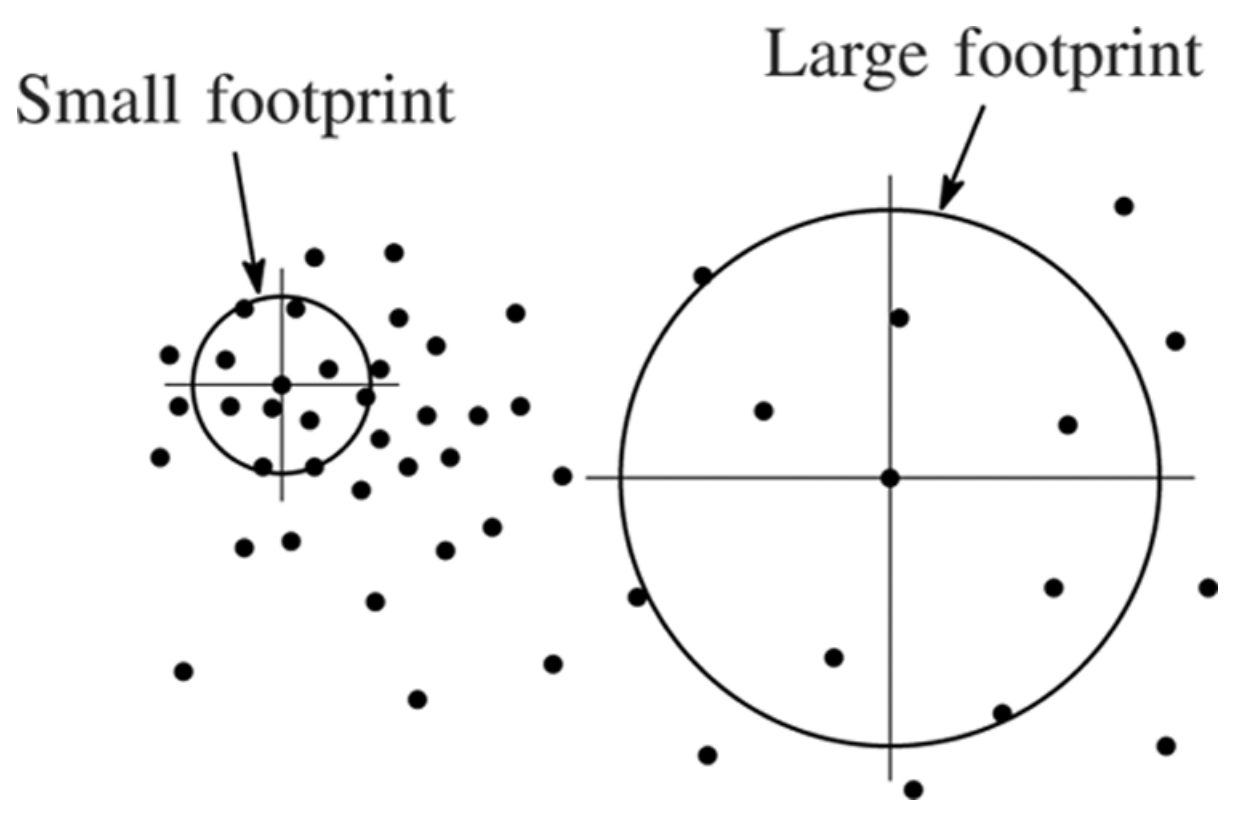
\includegraphics[width=.8\linewidth]{figures/classical/footprint.png}
    \caption{Kernel footprint as a function of sample density \cite{Takeda2007}.}
    \label{fig:footprint}
\end{figure}
\begin{figure}
    \centering
    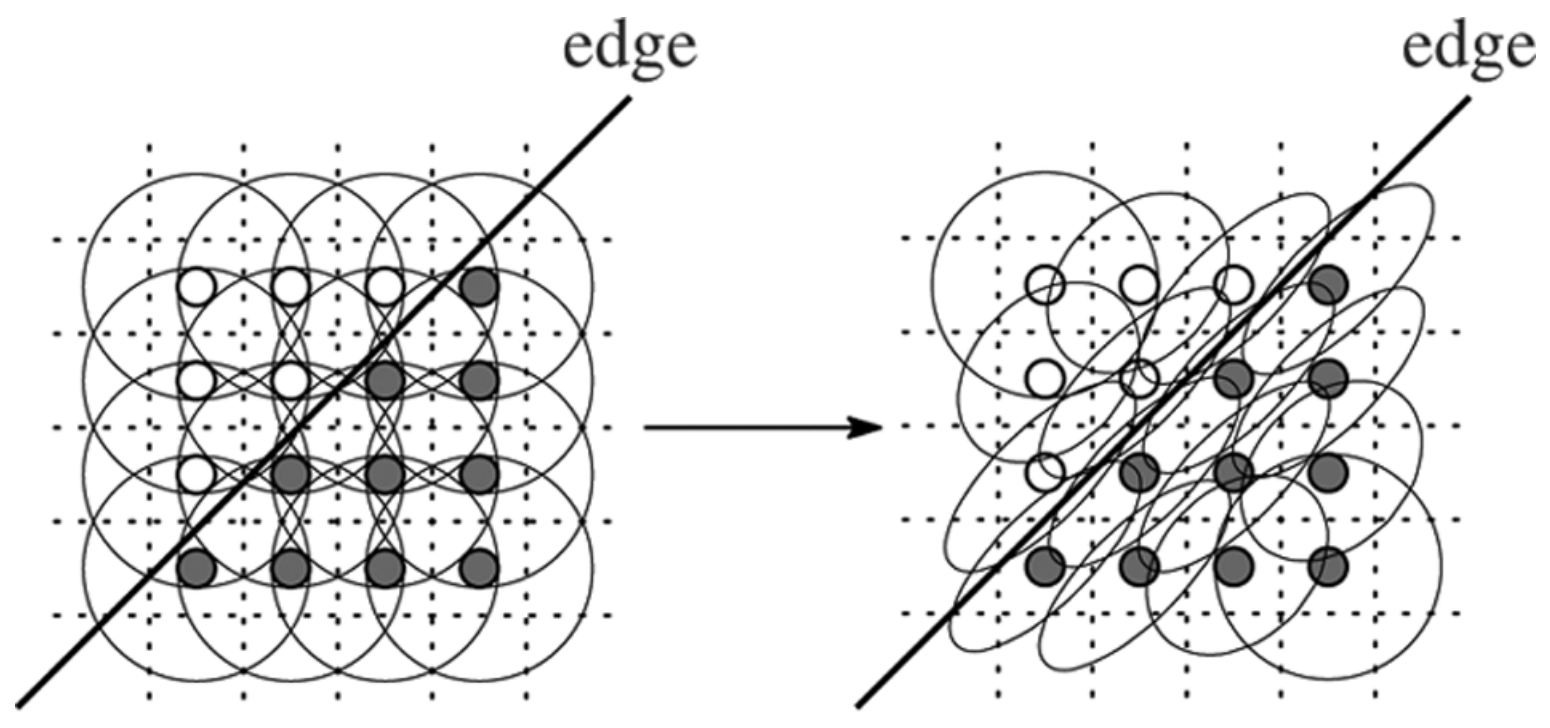
\includegraphics[width=\linewidth,keepaspectratio]{figures/classical/steering.png}
    \caption{Adapting kernel shape as a function of local directed structure \cite{Takeda2007}.}
    \label{fig:steering}
\end{figure}
In conventional kernel regression \(K\) might be any non-negative, symmetric, unimodal \cite{wand1994kernel} function with augmented with an additional \(h\) parameter that controls the bandwidth" or "footprint of the kernel, i.e.,\begin{equation}
    K_h(\delx) \coloneqq \frac{1}{h}K\left( h^{-1}(\delx) \right)
\end{equation}
This bandwidth parameter \(h\) can be generalized to a \textit{smoothing kernel} \(H\) in order to make \(K = K_H\) adaptive to the local structure of the pixels, e.g. to have larger footprints in sparsely sampled regions and have smaller footprints in densely sampled regions (see figure~\ref{fig:footprint}).
%
Ultimately though it is desirable to have kernels that can adapt to directed structure in the image, i.e.,steerable kernels that filter strongly along an edge and weakly across an edge.
%
This is accomplished by, for example, using a Gaussian as the kernel:
\begin{equation}
    K_{H_i}(\delx) \propto \frac{\exp\left\{ -(\delx)^T H^{-1}_i (\delx) \right\}}{\sqrt{\det{H_i}}}
\end{equation}
and identifying \(H_i\) with \(\nabla^2 \zbxi\) (since gradients capture edge structure).
%
An estimate \(\hat{H}_i\) of \(\nabla^2 \zbxi\) can be obtained by looking at covariances of empirical gradients (i.e.,the HR grid registered image convolved with a difference filter).
%
Unfortunately this is a naive estimate that is often rank deficient or unstable (both leading to instances where \(\hat{H}_i\) isn't invertible).
%
One solution is to parameterize \(H_i\):
\[
    H_i = \gamma_i U_{\theta_i} \Lambda_{\sigma_i} U_{\theta_i}^T
\]
where \(U_{\theta_i}\) is a rotation matrix, \(\Lambda_{\sigma_i} \coloneqq \text{diag}\left( \sigma_i, \sigma_i^{-1} \right)\) is an elongation matrix, and \(\gamma_i\) is a scaling parameter, with each of \(\gamma_i, \theta_i, \sigma_i\) estimated from the data in a more robust way.
%
\subsubsection{Bilateral Kernel}
An alternative kernel is the bilateral kernel \cite{Tomasi:1998:BFG:938978.939190} that defines closeness according to geometric and radiometric distance:
\begin{equation}
    \begin{split}
        K_S(\delx) &\coloneqq \exp \left\{ -\frac{\abs{ \delx }^2}{2 \sigma_S^2}  \right\} \\
        K_R(\bx, \bxi) &\coloneqq \exp \left\{ -  \frac{\abs{ Y(\bx) - Y(\bxi) }^2}{2 \sigma_R^2} \right\} \\
        K_B(\bx, \bxi) &\coloneqq K_S(\delx)K_R(\bx, \bxi)
    \end{split}
    \label{eqn:bilateralkernel}
\end{equation}
where \(\sigma_S\) parameterizes spatial distance weight and \(\sigma_R\) parameterizes radiometric distance weight.

In general non-uniform interpolation techniques are intuitive and typically (relatively) computationally efficient but they assume an unrealistic observation model (namely that of affine motion).

\subsection{Estimation}\label{subsec:estimation}

Statistical estimation methods cast SR as an inference problem.
%
\subsubsection{Iterative Back-Projection}\label{subsubsec:iterback}
One of the earliest successful SR algorithms \cite{Irani1991ImprovingRB} proposed an iterative scheme inspired by the back-projection method commonly used to reconstruct 2-D objects from 1-D projections in computer-aided tomography.
%
Recall eqn.~\eqref{eqn:imagingmodel}.
\begin{figure}
    \centering
    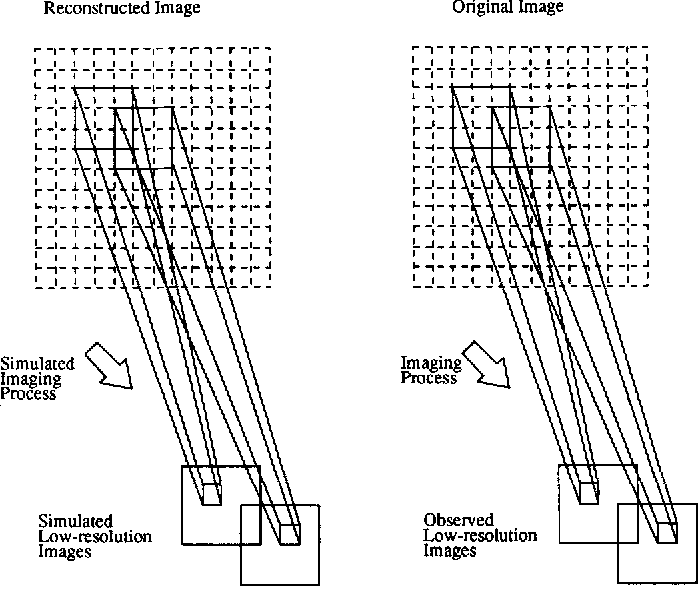
\includegraphics[width=\linewidth,keepaspectratio]{figures/classical/iterative_back_projection.png}
    \caption{Iterative back projection \cite{Irani1991ImprovingRB}.}
    \label{fig:iterbackproj}
\end{figure}
%
Then the idea is to take the current estimate of the HR image \(\hat{Y}^{i}\), see if after motion and down-sampling \((D \circ A_k)(\hat{Y}^i)\) it is near the LR samples \(\Xk\), and add a correction when it is not (see figure~\ref{fig:iterbackproj}):
\begin{equation}
    \hat{Y}^{i+1} = \hat{Y}^i + \sum_{k=1}^K (D \circ A_k)^{-1}\left( (D \circ A_k)(\hat{Y}^i) - \Xk \right)
    \label{eqn:ibp}
\end{equation}
where \(\hat{Y}^i\) is the current estimate of the blurred HR image, \((D \circ A_k)(\hat{Y}^i)\) is the projection of the current estimate to low resolution, and \((D \circ A_k)^{-1}\left( (D \circ A_k)(\hat{Y}^i) - \Xk \right)\) is the \textit{back-projection}.
%
This process iterates until convergence i.e.,\(\lvert (D \circ A_k)(\hat{Y}^i) - \Xk \rvert < \delta\) for some \(\delta\).
%
Irani \etal \cite{Irani1991ImprovingRB} also convolve the back-projection with a smoothing kernel as a form of regularization since the estimation problem is in general ill-posed (there are many \(\hat{Y}^{i}\) that will project down to a pixel-distance neighbor of \(\Xk\)).
%
It can be shown \cite{Elad1996} that for \(\varepsilon_k\) distributed \((0, R_k)\)-Normal, \(\hat{Y}\) is none other than the maximum likelihood MLE for \(Y\).
%
We can see this by recognizing that eqn.~\eqref{eqn:ibp} is just the Richardson iterative \cite{Anderssen:1972:RNM:891962} solution to the unconstrained optimization problem
\begin{equation}
    L(Y) = \frac{1}{2} \abs{ \bm{X} -  \begin{bmatrix}
            D_1 \circ A_1 \\
            D_2 \circ A_2 \\
            \vdots        \\
            D_K \circ A_K \\
        \end{bmatrix}  Y  }^2
    \label{eqn:l2regression}
\end{equation}
since
\begin{equation*}
    \nabla_{Y} L = 0
    \iff
    \sum_{k=1}^K (D \circ A_k)^{-1}\left( (D \circ A_k)(Y) - \Xk \right) = 0
\end{equation*}
and therefore \(\hat{Y}_i \rightarrow \hat{Y}\) is the MLE (since MLE is the solution to least squares \cite{CaseBerg:01}).
%
Though this is one of the oldest SR algorithms it's recently been revisited and re-imagined as a deep neural network architecture (DNN) \cite{haris2018deep} (see section~\ref{subsubsec:dbpn}).
\subsubsection{Kalman Filter}
Another estimation technique employs a Kalman filter \cite{elad1999} to estimate \(Y\).
%
Let \(\bm{x}_k = \text{vec}(\Xk)\) be the vectorization\anote{vectorize} of \(\Xk\) and \(\bm{y} = \text{vec}(Y)\) likewise.
%
If we assume linear models for each of \(D, A_k, H_k\) (i.e.,all representable as matrices) and a well-behaved motion model (most pixels in image \(\bm{x}_k\) appear in image \(\bm{x}_{k-1}\)) then we can image \(\bm{y}\) as a sequence of images \(\bm{y}_k\) related in time by
\begin{equation}
    \bm{y}_k = A'_k \bm{y}_{k-1} + \eta_k
    \label{eqn:kalmanprocess}
\end{equation}
%
where \(A'_k\) is the \textit{relative} motion operator, \(A'_k\bm{y}_{k-1}\) is conventional matrix-vector multiplication, and \(\eta_k\) is the only source of new pixels (noise\anote{noise} distributed \((0, Q_k)\)-Normal).
%
Consequently eqn.~\eqref{eqn:imagingmodel} becomes
\begin{equation}
    \bm{x}_k = DH_k\bm{y}_k + \varepsilon_k
    \label{eqn:kalmanobs}
\end{equation}
and the pair of eqns.~\eqref{eqn:kalmanprocess},~\eqref{eqn:kalmanobs} can be seen to constitute a linear dynamical system with \(\bm{y}_k\) the state of the system, \(A'_k\) the state transition, \(\eta_k\) the state noise, \(\bm{x}_k\) the measurement, \(DH_k\) the measurement model, and \(\varepsilon_k\) the measurement noise.
%
Note that the HR image conditioned on all previous LR images (measurements)
\begin{equation}
    \bm{y}_{k|s} \coloneqq \bm{y}_k|\bm{x}_1, \mathellipsis, \bm{x}_s
\end{equation}
where \(s \leq k\), is a GP, with mean \(\bar{\bm{y}}_{k|s} = E\left[\bm{y}_{k|s}\right]\)
and covariance
\begin{equation}
    C_{k|s} \coloneqq E\left[ (\bm{y}_k - \bar{\bm{y}}_{k|s})(\bm{y}_k - \bar{\bm{y}}_{k|s})^T  \right]
\end{equation}
%
By definition the MMSE \(\hat{\bm{y}}_{k|s}\) of \(\bm{y}_{k|s}\) is \(\bar{\bm{y}}_{k|s}\) and therefore \(C_{k|s}\) is the covariance of the error of the estimate \(\hat{\bm{y}}_{k|s}\).
%
The Kalman filter proceeds in two steps: an \textit{a priori} (before measurement) prediction step and an \textit{a posteriori} (after measurement) update step.
%
The prediction step iterates on the estimate (and its covariance) given all previous measurements:
\begin{align}
    \hat{\bm{y}}_{k|k-1} & = A'_k \hat{\bm{y}}_{k-1|k-1}     \\
    C_{k|k-1}            & = A'_k C_{k-1|k-1} (A'_k)^T + Q_k
\end{align}
This can be seen as a one-step propagation of the estimate in the direction of the previous measurement.
%
Then the update step incorporates new information from a measurement:
\begin{align}
    \hat{\bm{y}}_{k|k} & = \hat{\bm{y}}_{k|k-1} + K_k(\bm{x}_k - DH_k\hat{\bm{y}}_{k|k-1} ) \\
    C_{k|k}            & = (I - K_k DH_k)C_{k|k-1}
\end{align}
where the \text{Kalman gain}
\begin{equation}
    K_k \coloneqq \frac{C_{k|k-1}(DH_k)^T}{DH_k C_{k|k-1} (DH_k)^T + R_k }
\end{equation}
weights the contribution of the prediction and the measurement\anote{kalmanprediction}.
%
Note that in the Kalman framework \(D, H_k, A'_k, R_k, Q_k\) are all assumed to be known.
%
In Elad \etal \cite{elad1999} the assumption is \(D, H_k, R_k\) are known functions of camera parameters, \(A'_k\) can be estimated by an image registration algorithm and \(Q_k\) can be approximated:
\begin{equation}
    Q_k \approx \alpha_k A'_k C_{k|k} (A'_k)^T
\end{equation}
where \(\alpha_k\) is chosen such that the approximation upper-bounds the true \(Q_k\).
%
They comment that this stronger auto-correlation for \(\bm{y}_k\) adds pseudo-noise" to the system and biases the Kalman filter to "rely more on the measurements than the state transition model.
\subsubsection{MAP Estimation}
SR can also be posed as a Bayesian maximum a posterior (MAP) estimation problem.
%
Let \(\bm{H} \coloneqq \left( H_1, \mathellipsis, H_k \right)\) be the vector of blur operators applied to \(Y\) in order to produce \(\bm{X}\) and similarly \(\bm{A}\).
%
Then
\begin{align}
    \hat{Y} & \coloneqq \underset{Y}{\text{argmax}}~P\left( Y \middle| \bm{X} \right) \nonumber                                                                                        \\
            & = \underset{Y}{\text{argmax}} \int_{D, \bm{H}, \bm{A}} P\left( Y, D, \bm{H}, \bm{A} \middle| \bm{X}\right) \nonumber                                                     \\
            & = \underset{Y}{\text{argmax}} \int_{D, \bm{H}, \bm{A}} \frac{P\left(\bm{X} \middle| Y, D, \bm{H}, \bm{A} \right)P(Y) P(D, \bm{H}, \bm{A})}{P(\bm{X})}\label{eqn:indepym} \\
            & = \underset{Y}{\text{argmax}} \int_{D, \bm{H}, \bm{A}} P\left(\bm{X} \middle| Y, D, \bm{H}, \bm{A} \right)P(Y) P(D, \bm{H}, \bm{A}) \label{eqn:maxx}
\end{align}
where in eqn.~\eqref{eqn:indepym} we've used the independence of \(Y\) and \(D, \bm{H}, \bm{A}\) \cite{Hardie1997} and in eqn.~\eqref{eqn:maxx} we've used that \(\bm{X}\) is a constant with respect to the maximization.
%
While there exist reasonable priors for \(Y\), marginalizing over \(D, \bm{H}, \bm{A}\) is still difficult due to the high-dimensionality of each.
%
Therefore assuming \(D, \bm{H}, \bm{A}\) can be estimated independently as \(\hat{D}, \hat{\bm{H}}, \hat{\bm{A}}\), eqn.~\eqref{eqn:maxx} becomes
\begin{equation}
    \hat{Y} = \underset{Y}{\text{argmax}}~P\left(\bm{X} \middle| Y; \hat{D}, \hat{\bm{H}}, \hat{\bm{A}} \right) P(Y)
    \label{eqn:map}
\end{equation}
where the semicolon indicates \(\hat{D}, \hat{\bm{H}}, \hat{\bm{A}}\) are known parameters of the conditional distribution.
%
This casts \(\hat{Y}\) the standard MAP estimate of \(Y\).
%
Note that an equivalent formulation of MAP maximizes the log-likelihood instead of maximizing the likelihood:
\begin{align}
    \hat{Y} & = \underset{Y}{\text{argmax}}\left[ \log\left( P\left(\bm{X} \middle| Y; \hat{D},  \hat{\bm{H}}, \hat{\bm{A}}\right) P(Y) \right) \right]  \nonumber \\
            & =  \underset{Y}{\text{argmax}}\left[ \log{P\left(\bm{X} \middle| Y; \hat{D},  \hat{\bm{H}}, \hat{\bm{A}} \right)} + \log{P(Y)} \right]
    \label{eqn:logmap}
\end{align}
%
Various choices for \(P\left(\bm{X} \middle| Y; \hat{D},  \hat{\bm{H}}, \hat{\bm{A}} \right)\) and the prior \(P(Y)\) (and consequent choice of optimization strategies) characterize this class of SR techniques.
%
Again assume \(D, H_k, A_k\) linear and given \(\varepsilon_k\) in eqn.~\eqref{eqn:imagingmodel} distributed \((0, rI)\)-Normal
\begin{equation}
    P\left(\bm{X} \middle| Y; \hat{D},  \hat{\bm{H}}, \hat{\bm{A}} \right) \propto \exp \left\{ -\frac{\abs{ \bm{X} - \hat{D} \hat{\bm{H}} \hat{\bm{A}} \bm{y} }^2}{2r^2} \right\}
\end{equation}
where here \(\bm{X} \coloneqq \left( \text{vec}(X_1), \mathellipsis, \text{vec}(\Xk) \right)\) and
\begin{equation}
    \hat{D} \hat{\bm{H}} \hat{\bm{A}} \coloneqq \begin{bmatrix}
        \hat{D} \hat{\bm{H}}_1 \hat{\bm{A}}_1 \\
        \hat{D} \hat{\bm{H}}_2 \hat{\bm{A}}_2 \\
        \vdots                                \\
        \hat{D} \hat{\bm{H}}_K \hat{\bm{A}}_K \\
    \end{bmatrix}
\end{equation}
%
After a suitable choice for the prior it can be seen that eqn.~\eqref{eqn:logmap} is just regularized regression.
%
For example when choosing a Gibbs \cite{Hardie1997} distribution as the prior, i.e.,\begin{equation}
    P(Y) \propto e^{-\alpha B(Y)}
    \label{eqn:gibbs}
\end{equation}
where \(B(Y)\) is called the \textit{potential}, eqn.~\eqref{eqn:logmap} becomes
\begin{equation}
    \hat{\bm{y}} = \underset{\bm{y}}{\text{argmin}}\left[ \abs{ \bm{X} - \hat{D} \hat{\bm{H}} \hat{\bm{A}} \bm{y} }^2 +\lambda B(Y)\right]
    \label{eqn:minmap}
\end{equation}
where the aggregate regularization parameter \(\lambda\) absorbs \(\alpha\) from \(P(Y)\) and \(r\) from \(\varepsilon_k\).
%
There are many other choices for the prior in eqn.~\eqref{eqn:logmap}, whose effect is to bias the estimator \(\hat{\bm{y}}\) towards natural images.
%
Alternatively we can (and will) take eqn.~\eqref{eqn:minmap} as our starting point and explicitly choose the regularizer \(B(Y)\).

\subsubsection{Tikhonov Regularization}

One of the simplest priors is a \((0, Q)\)-Normal, where \(Q\) is symmetric positive definite\anote{positivedef} (PD) and captures the covariance of neighboring pixels.
%
This corresponds to the regularizer taking the form
\begin{equation}
    B(Y) = \by ^T Q \by
\end{equation}
where \(\by = \text{vec}(Y)\).
%
Since \(Q\) is symmetric PD eqn.~\eqref{eqn:minmap} becomes
\begin{equation}
    \hat{\bm{y}} = \underset{\bm{y}}{\text{argmin}}\left[ \abs{ \bm{X} - \hat{D} \hat{\bm{H}} \hat{\bm{A}} \bm{y} }^2 +\lambda \abs{ \sqrt{Q}\bm{y} }^2 \right]
    \label{eqn:tikminmap}
\end{equation}
where \(\sqrt{Q}\) is \(U\) of the Cholesky decomposition \(Q = U^T U\).
%
Equation~\ref{eqn:tikminmap} is Tikhonov regularized regression, or Ridge regression if \(\sqrt{Q} = I\).
%
Letting \(G = \hat{D} \hat{\bm{H}} \hat{\bm{A}}\) the closed-form solution to eqn.~\eqref{eqn:tikminmap} is
\begin{equation}
    \hat{\by} = \left( G^T G + \lambda Q \right)^{-1} G^T\bX
    \label{eqn:closedform}
\end{equation}
Nguyen \etal \cite{milanfar2001} use cross-validation to determine the regularization parameter \(\lambda\) (by partitioning the pixels into a fit" and "validate set).
%
In general, rather than explicitly computing inverses in eqn.~\eqref{eqn:closedform}, in practice \(\hat{\bm{y}}\) is found by solving the regression problem via optimization (for high-dimensional matrices optimization is faster than inversion).
%
Nguyen \etal use conjugate gradient descent\anote{conjugategradients} to optimize eqn.~\eqref{eqn:tikminmap}.
%
They argue that \(\hat{D} \hat{\bm{H}} \hat{\bm{A}}\) is ill-conditioned\anote{illcondition} and to that end, since the convergence rate of conjugate gradients is dependent on the condition number \cite{vanderSluis1986}, propose pre-conditioners\anote{precondition} to improve the converge rate.

\subsubsection{Huber Loss and TV Loss}\label{subsubsec:huberloss}

An issue with the multivariate Normal prior is that it strongly enforces global smoothness, penalizing sharp edges.
%
One solution is to use Huber loss \cite{huber1964}
\begin{equation}
    \mathcal{H}_{\delta }(a)\coloneqq {
        \begin{cases}
            a^2                                 & \text{for }\lvert a \rvert \leq \delta \\
            2 \delta \lvert a \rvert - \delta^2 & {\text{otherwise}}
        \end{cases}
    }
\end{equation}
to explicitly parameterize the penalty for gradients (i.e.,high-frequency features).
%
Huber loss enforces local smoothness (since it's quadratic for \(\lvert a \rvert \leq \delta\)) but permits edges (since it's linear for \(\lvert a \rvert > \delta\)).
%
Capel \etal \cite{capel2000} implement this by composing \(L_{\delta }(a)\) with a first-order gradient operator\anote{gradientoperator} as the potential in eqn.~\eqref{eqn:gibbs}.
%
Another gradient penalty that encourages sparse gradients (i.e.,local smoothness and steep edges) is Total Variation (TV) norm \cite{RUDIN1992259}:
\begin{equation}
    \abs{u}_{\operatorname {TV}}\,\coloneqq\int _{\Omega }\abs{\nabla u}\,d\Omega
\end{equation}
where \(u\) is a smooth image of bounded variation (i.e.,such that the integral converges) over domain \(\Omega\).
%
In the context of SR this amounts to setting
\begin{equation}
    B(Y) = TV(Y) \coloneqq \abs{ \nabla Y }_1
\end{equation}
%
Farsiu \etal \cite{farsiu} introduce a \textit{bilateral} TV norm
\begin{equation}
    BTV(Y) \coloneqq \sum_{k=0}^{N} \sum_{l=0}^{N} \alpha^{k + l} \abs{ Y - S_x^k S_y^l Y }_1
\end{equation}
where \(S_x^k, S_y^l\) are shift operators (i.e.,\(S_x^k\) shifts \(Y\) by \(k\) pixels in the horizontal) and \(N\) is arbitrary.
%
The bilateral TV norm factors in gradients at several scales (\(Y - S_x^2 Y\) is an approximation of the horizontal gradient at twice the scale of \(Y - S_x^1 Y\)) and decays their contribution according to their spatial distance (\(\alpha^{k+l}\) decays as a function of shift distance).
%
It can also be shown to be equivalent \cite{elad2002} to filtering \(\bX\) by the bilateral kernel (see eqn.~\eqref{eqn:bilateralkernel}).

Though there are many priors (or regularizers) that have been studied none really capture natural images in all of their variation.
%
For that we need to actually learn from real data i.e.,examples images.

\subsection{Example based}\label{subsec:example-based}

Example based techniques \textit{learn} a mapping from
LR patches to HR patches based on a training set and then use that mapping to predict details in new (unseen) images.

\subsubsection{Hidden Markov Random Field}

Freeman \etal \cite{freeman2002example} argues that the most important features to reconstruct are the high-frequency features.
%
Therefore they store only the correspondence between high-pass filtered, contrast-normalized versions of example LR patches and HR patches.
%
Note that they pre-process the LR images by cubic-spline interpolating to the higher pixel sampling resolution and that HR patches are sampled to overlap by one or more pixel widths at their edges.
%
Naive mosaicing of these matching HR patches produces poor results due to noise and the ill-posed nature of super-resolution.
%
\begin{figure}
    \centering
    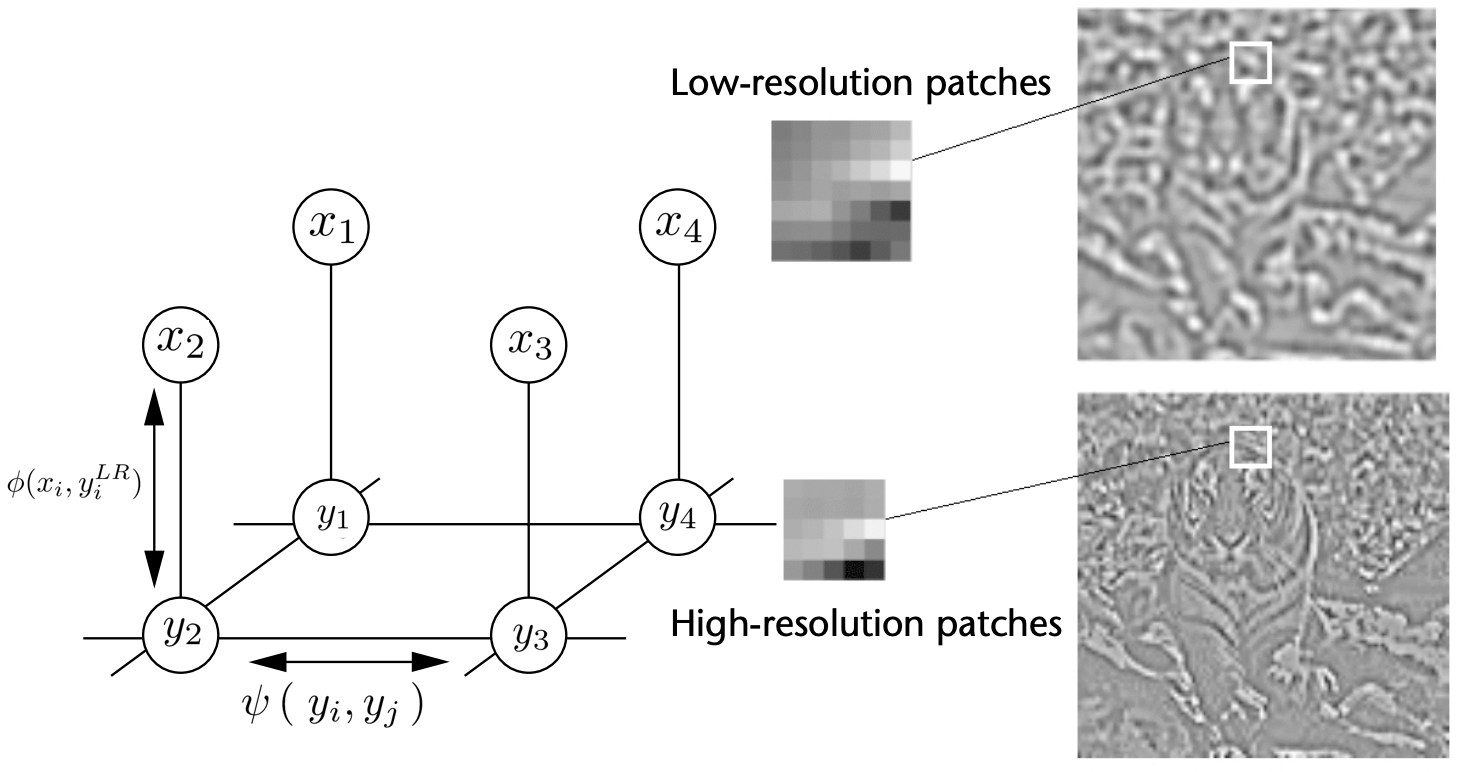
\includegraphics[width=\linewidth,keepaspectratio]{figures/classical/mrf.png}
    \caption{Hidden Markov random field modeling spatial relationships between LR patches \(x_i\) and example LR patches \(y_i^{LR}\) and HR patches \(y_i\) \cite{freeman2002example}.}
    \label{fig:mrf}
\end{figure}
Their solution to this issue is using a hidden Markov random field\anote{hmrf} (HMRF) to model spatial consistency between adjacent HR patches \(y_i\) and between LR-HR patch pairs \(x_i, y_i\) (see figure~\ref{fig:mrf}).
%
They then compute the MAP estimate of the HMRF to obtain the smoothest assignment of HR patches: the HMRF model postulates that the conditional probability of any HR patch assignment \(\by\) given observed LR patches \(\bx\) is
\begin{equation}
    P\left( \by \middle| \bx \right) = \frac{1}{P(\bx)} \prod_{i\ue{} j} \psi(y_i, y_j) \prod_i \phi(x_i, y_i^{LR})
\end{equation}
where \(x_i\) are observed LR patches and \(y_i\) are unknown (to-be-inferred) HR patches (along with their learned-mapping example LR patches \(y_i^{LR}\)).
%
Note \(P(\bx)\) is a normalization constant, \(i\ue{} j\) indicates the product is only over adjacent HR patches, \(\psi(y_i, y_j)\) encodes the compatibility of adjacent HR patches according to
\begin{equation}
    \psi(y_i, y_j) \coloneqq \exp \left\{ -  \frac{\abs{ y_i - y_j }}{2\sigma^2} \right\}
\end{equation}
where \(\abs{ y_i - y_j }\) is only computed on the overlapping pixels.
%
Similarly \(\phi(x_i, y_i^{LR})\) encodes the compatibility between the observed LR patch \(x_i\) and the example LR patch \(y_i^{LR}\) corresponding to the estimated HR patch \(y_i\).
%
To make the MAP computation tractable they choose only 16 candidate example LR patches \(y_i^{LR}\).
%
They compute the MAP estimate using belief propagation\anote{beliefpropagation}.

\subsubsection{Nearest Neighbor Embedding}
An issue with the direct LR-HR patch pair technique is that it requires an enormous database of patches in order for it to generalize.
%
\begin{figure}
    \centering
    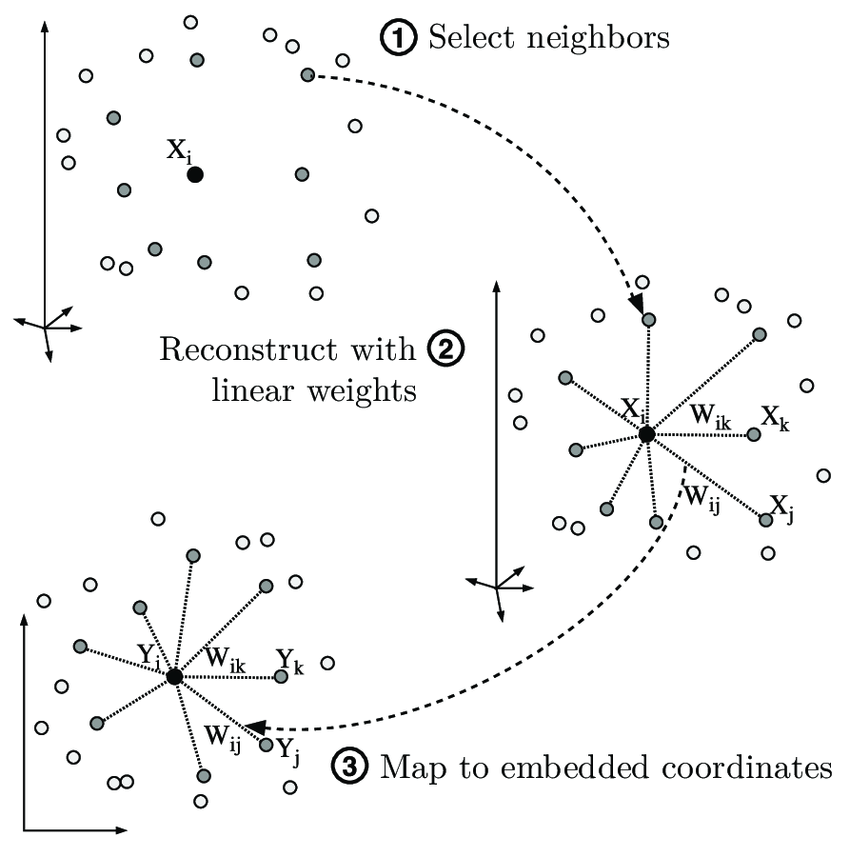
\includegraphics[width=\linewidth,keepaspectratio]{figures/classical/lle.png}
    \caption{NNE algorithm from LR patches \(x_i\) to HR patches \(y_i\) \cite{Guillermophdthesis}.}
    \label{fig:lle}
\end{figure}
Chang \etal remedy this problem by using ideas from a manifold\anote{manifold} learning\anote{manifoldlearning} technique called locally linear embedding \cite{saul2000introduction} (LLE) that they call nearest neighbor embedding (NNE).
%
First they imagine both the space of LR patches and HR patches as manifolds.
%
Then based on the intuition that a well-sampled smooth manifold is locally linear (i.e.,an LR patch \(x_i\) on the LR manifold and its neighbors \(x_j, x_k, \mathellipsis\) lie in a locally linear subspace of the manifold) they characterize the local geometry.
%
One can characterize local geometry by finding convex reconstruction weights \(W_{ij}\) of any \(x_i\) from only its neighbors by minimizing reconstruction error, i.e.,\begin{gather}
    \hat{W} \coloneqq \underset{W_{ij}}{\text{argmin}} \sum_i \abs{ x_i - \sum_{x_j \in N(x_i)} W_{ij} x_j  }^2 \nonumber \\
    \text{s.t.} \\
    \sum_{x_j \in N(x_i)} W_{ij} = 1 \text{ for all }i \nonumber
\end{gather}
where \(N(x_i)\) is the neighborhood of \(x_i\).
%
These weights \(W_{ij}\) are invariant with respect to rotation, rescaling, and translation of the LR patch and its neighborhood \cite{saul2000introduction} and therefore should remain valid in an embedding space (i.e.,the HR manifold) coordinate system (see figure~\ref{fig:lle}).
%
The HR patches \(y_i\) in the HR manifold are then reconstructed using the same weights, i.e.,
\begin{equation}
    y_i = \sum_{x_j \in N(x_i)} W_{ij} y_j
\end{equation}
%
Note that neighboring patches in HR space are constrained to overlap and in fact the neighborhoods are computed using gradient features of the LR and HR patches rather than the raw patches.
%
Chang \etal argue that this is what allows for better generalization i.e., much smaller patch databases.

\subsubsection{Sub-Band Energy Attenuation}\label{subsubsec:subband}
Another issue with using LR-HR patch pairs to train NNE is the uncertainty associated with matching highly textured patches, i.e., those with large gradients.
%
Zontak \etal \cite{zontak2011internal} show that finding matches between image patches becomes more and more unlikely as the mean gradient magnitude per patch increases.
%
This is directly as a result of the fact that \(L_2\) distances between patches are primarily determined by prominent image structures.
%
Singh \etal \cite{singh2014} make this intuition rigorous by decomposing HR and SR patch pairs into oriented \textit{sub-bands} (i.e., gradient orientation bins) and demonstrating that low-energy sub-bands (i.e., those that contribute weakly to the decomposition) are more strongly attenuated (see figure~\ref{fig:subbands}).
\begin{figure}
    \centering
    \begin{adjustbox}{width=\linewidth}
        \centering
        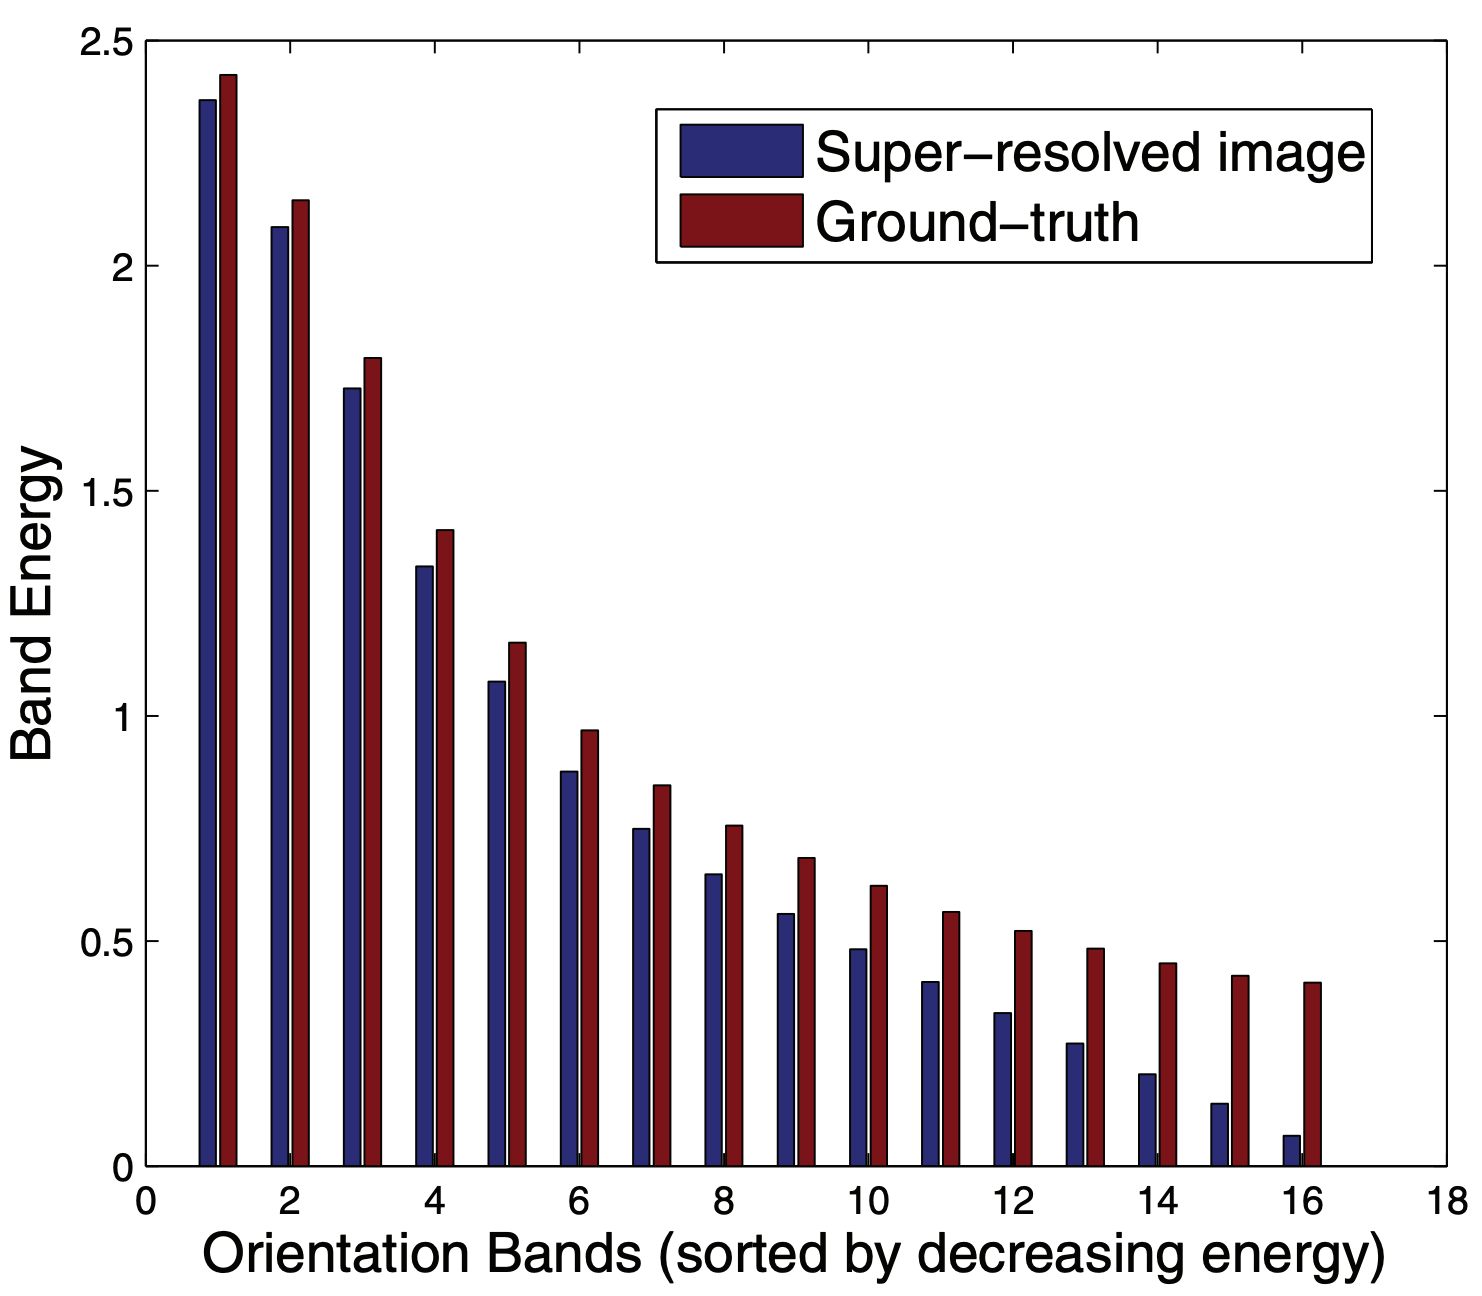
\includegraphics{figures/classical/subbands.png}
    \end{adjustbox}
    \caption{Oriented gradient attentuation sorted by energy \cite{singh2014}.}\label{fig:subbands}
\end{figure}
To mitigate the effect of this insensitivity of the \(L_2\) metric, they learn the necessary gains to apply in order to recover such low energy patches (along with the matchings).

\subsubsection{Sparse Coading}\label{subsubsec:sparsecoding}
NNE also suffers from using a fixed number of nearest neighbors results in blurring (due to over-fitting or under-fitting).
%
Yang \etal \cite{yang2008} resolve this issue by using sparse coding (SC) as a framework for learning a sparse mapping from LR patches to HR patches (see figure~\ref{fig:hrpatchdict}).
%
This enables them to essentially leave the number of nearest numbers unspecified (or, alternatively, learn the correct number of neighbors on a patch by patch basis\anote{pun}).
%
To be precise, let \(D \in \mathbb{R}^{n \times K}\) be an \textit{over-complete dictionary}\anote{overcompletedictionary} of \(K\) atoms \(\bm{d}_i \in \mathbb{R}^n\), and suppose a signal \(\by \in \mathbb{R}^n\) can be represented as a sparse linear combination of these atoms i.e.,\begin{equation}
    \by = D\bm{\alpha}
\end{equation}
such that \(\abs{ \bm{\alpha} }_0 \ll K\) (few non-zero entries).
%
The sparse vector \(\bm{\alpha}\) is variously called the code, reconstruction, or sparse representation of \(\by\).
%
Yang \etal construct two dictionaries \(D_{LR}, D_{HR}\) consisting corresponding LR and HR patches \(\bxi, \byi\).
%
Then given a new input LR patch \(\bx\) they compute the code for a featurized representation of \(\bx\) in \(D_{LR}\) by minimizing the code subject to reconstruction error tolerance:
\begin{equation}
    \hat{\bm{\alpha}} \coloneqq \underset{\bm{\alpha}}{\text{argmin}} \abs{ \bm{\alpha} }_0 \text{ s.t. } \abs{ F\bx - FD_{LR}\bm{\alpha} }^2 \leq \epsilon
    \label{eqn:constrainedrepr}
\end{equation}
where \(\epsilon\) is the reconstruction error tolerance and \(F\) is the feature extraction operator (first and second order gradients), and construct the HR image using the same sparsely represented HR patch (i.e.,\(\hat{\by} = D_{HR} \hat{\bm{\alpha}}\)).
%
As stated the optimization in eqn.~\eqref{eqn:constrainedrepr} is non-convex (due to \(\abs{ \bm{\alpha} }_0\)) and is in fact NP-hard\anote{nphard} \cite{tilman2015}.
%
Fortunately the \(L_1\) (i.e.,\(\abs{ \bm{\alpha} }_1\)) relaxation is often good enough \cite{Donoho9446}:
\begin{equation}
    \hat{\bm{\alpha}} = \underset{\bm{\alpha}}{\text{argmin}} \left[ \lambda\abs{ \bm{\alpha} }_1 + \frac{1}{2}\abs{ F\bx - FD_{LR}\bm{\alpha} }^2 \right]
    \label{eqn:lagrangerepr}
\end{equation}
where we've also transformed to the unconstrained optimization using the Lagrange multiplier \(\lambda\).
%
Solving eqn.~\eqref{eqn:lagrangerepr} input-patch by input-patch does not enforce consistency between adjacent patches.
%
They use a raster-scan technique discussed in Freeman \etal \cite{freeman2002example} to enforce consistency.
%
They further comment that since eqn.~\eqref{eqn:constrainedrepr} doesn't demand equality between the LR patch \(\bx\) and its reconstruction \(D_{LR}\bm{\alpha}\) the reconstructed image \(Y\) might not satisfy the imaging model (see eqn.~\eqref{eqn:imagingmodel}).
%
They resolve this by using iterative back projection (see eqn.~\eqref{eqn:ibp}) as a final step in the algorithm.
%
While the sparse representation approach mitigates issues having to do with local bias (fixed number \(K\) patch neighbors) it still requires a large database of raw image patches.
%
The same group's follow-on paper \cite{yang2010} addresses this issue directly by learning the LR, HR dictionaries with a fixed number of atoms \(K\).
\begin{figure}
    \centering
    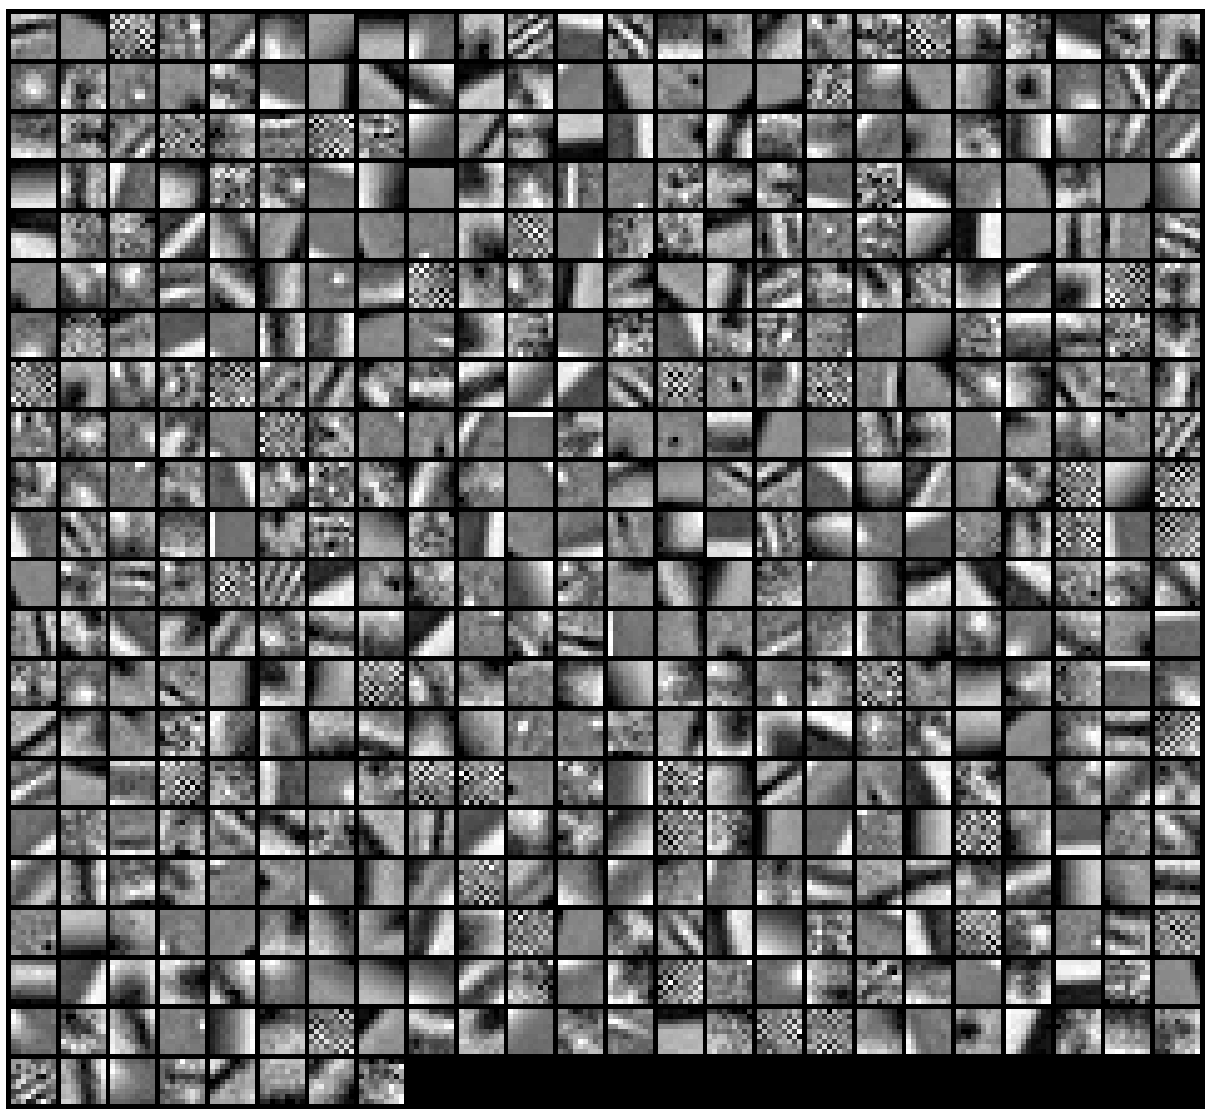
\includegraphics[width=\linewidth,keepaspectratio]{figures/classical/dictpatches.png}
    \caption{512 entry \(9 \times 9\) atom HR image patch dictionary trained using 100,000 HR and LR image patch pairs \cite{yang2010}.}
    \label{fig:hrpatchdict}
\end{figure}
%
In general dictionary learning minimizes the reconstruction error of the codes across all \(J\) example inputs \(\bm{Z} \coloneqq \left( \bm{z}_1, \mathellipsis, \bm{z}_J \right)\):
\begin{equation}
    \hat{D} \coloneqq \underset{D, \bm{A}}{\text{argmin}} \abs{ \bm{Z} - D\bm{A} }^2 + \lambda \abs{ \bm{A} }_1
\end{equation}
where \(\bm{A} \coloneqq \left( \bm{\alpha}_1, \mathellipsis, \bm{\alpha}_J  \right)\).
%
Yang \etal jointly learn \(D_{LR}, D_{HR}\) by making the identifications
\begin{equation*}
    \bm{Z} \coloneqq \begin{bmatrix}
        \frac{1}{\sqrt{N}}\bY \\ \frac{1}{\sqrt{M}} \bX
    \end{bmatrix} \text{ and }
    D \coloneqq \begin{bmatrix}
        \frac{1}{\sqrt{N}} D_{HR} \\ \frac{1}{\sqrt{M}} D_{LR}
    \end{bmatrix}
\end{equation*}
where \(\bY \coloneqq \left( \by_1, \mathellipsis, \by_P \right)\) are the example HR patches, \(\bX\) similarly the example LR patches, and \(N, M\) are the number of HR and LR pixels respectively in each example patch pair \(\byi, \bxi\) (in order to normalize the error between \(\byi, \bxi\)).

\subsubsection{Anchored Neigbhorhood Regression}
Though SC achieves good results for reasonably sized example sets and dictionary sizes it suffers from the inherent computational complexity of solving the optimization problem (see figure~\ref{fig:dictspeedspize}).
\begin{figure}
    \centering
    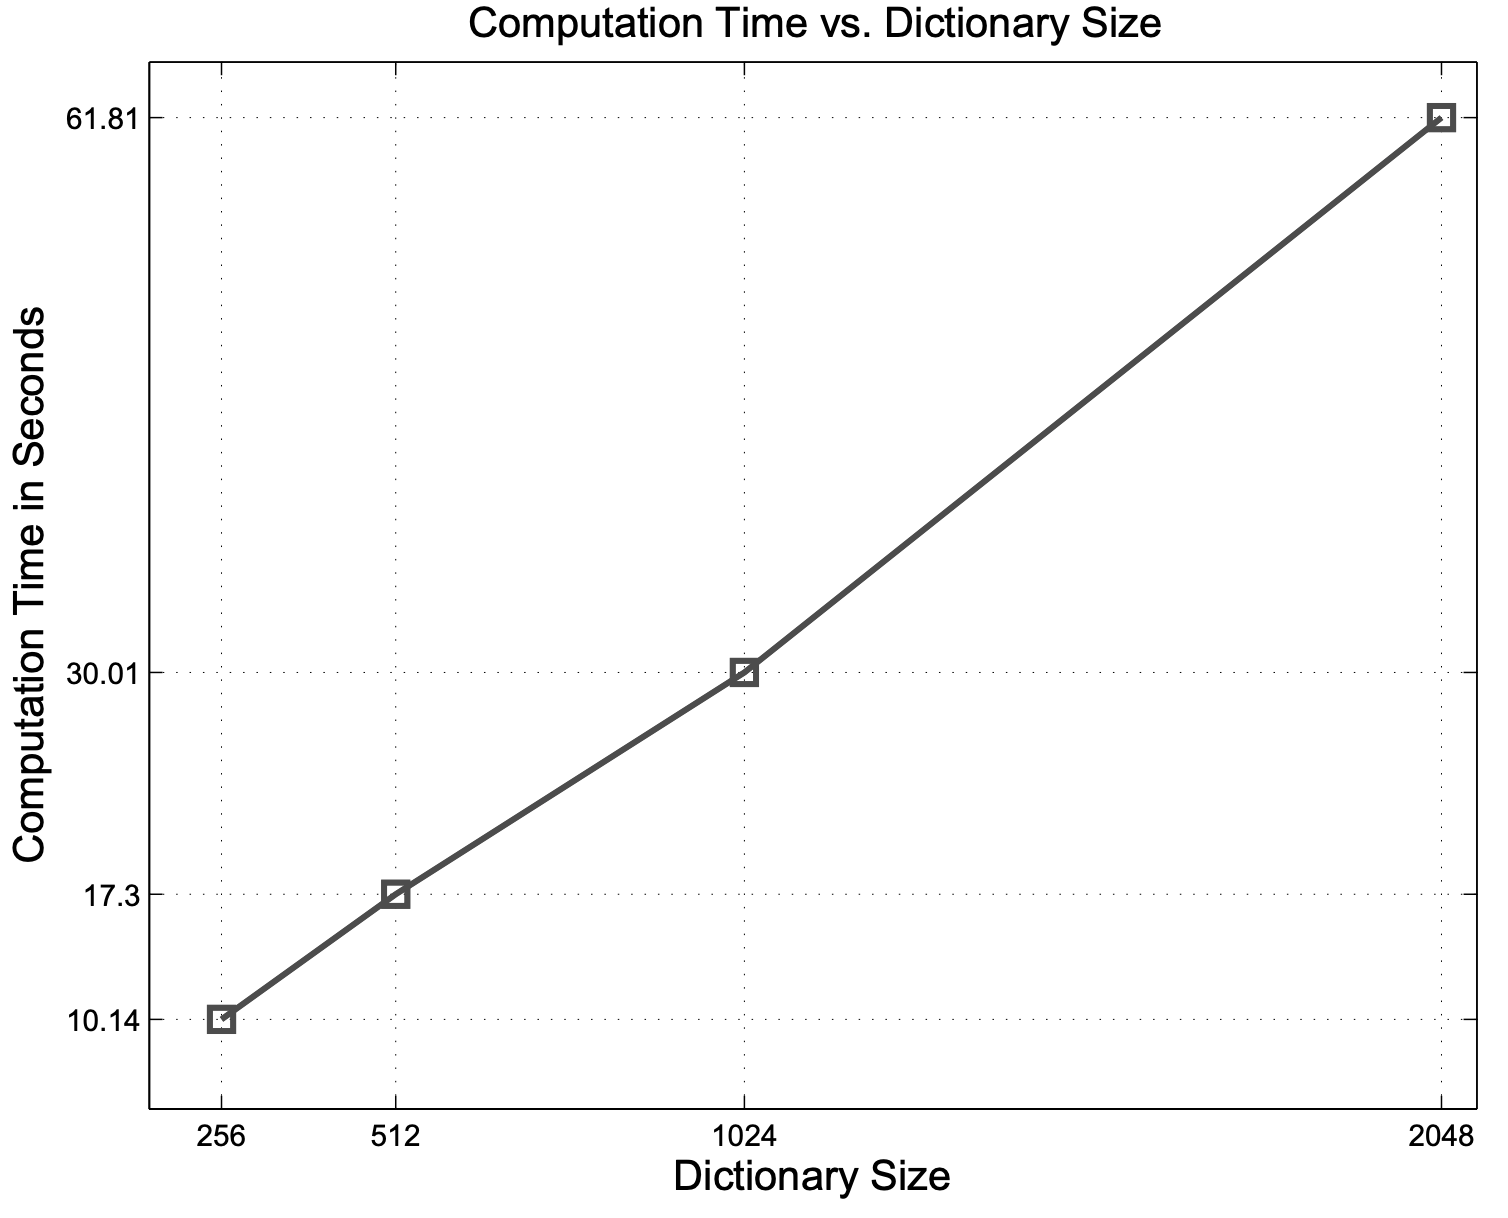
\includegraphics[width=\linewidth,keepaspectratio]{figures/classical/dictsizespeed.png}
    \caption{Dictionary inference time as a function of dictionary size \cite{yang2010}.}
    \label{fig:dictspeedspize}
\end{figure}
%
Timofte \etal \cite{Timofte} argues that the chief inefficiency is the \(L_1\) norm on the code.
%
By relaxing the \(L_1\) norm in eqn.~\eqref{eqn:lagrangerepr} to the \(L_2\) norm they recover the Ridge regression form of the problem (see eqn.~\eqref{eqn:closedform}) and get a closed form solution for the code:
\begin{equation}
    \hat{\bm{\alpha}} = \left( D_{LR}^T D_{LR} + \lambda I\right)^{-1}D_{LR}^T \bx
\end{equation}
The code can then be used to compute the HR patch:
\begin{align}
    \by & = D_{HR} \hat{\bm{\alpha}}                                                               \\
        & = D_{HR} \left( D_{LR}^T D_{LR} + \lambda I\right)^{-1}D_{LR}^T \label{eqn:mappinglr}\bx
\end{align}
Factoring out
\begin{equation}
    P \coloneqq D_{HR} \left( D_{LR}^T D_{LR} + \lambda I\right)^{-1}D_{LR}^T
\end{equation}
we see that \(P\) can be pre-computed, thereby turning inference into simply a matrix multiplication.
%
They then go on to argue, reasoning by analogy with NNE, that the projection should be locally sensitive to input patches, i.e.,instead of using the entire dictionary to construct the projection only the atoms nearest to the input LR patch should be used.
%
Thus for every atom in the dictionary, they find its \(K' < K\) nearest neighbors, and using only those \(K'\) atoms they pre-compute \(K\) distinct projection operators \(P_k \in \mathbb{R}^{n \times K'}\):
\begin{equation}
    P_k \coloneqq D_{HR}^k \left( (D_{LR}^k)^T D_{LR}^k + \lambda I\right)^{-1}(D_{LR}^k)^T
    \label{eqn:datadependentmapping}
\end{equation}
where \(D_{LR}^k, D_{HR}^k\) are the neighborhood of the LR atom and the neighborhood of its corresponding HR atom.
%
They call these \(P_k\) \textit{anchored regressions} because they effectively weight the contributions of LR and HR dictionary atoms.
%
For a new input LR patch \(x\) they find the nearest atom in the \(D_{LR}\) and recover the HR patch \(\by = P_k \bx\).
%
Note that ANR, just as in SC, does not operate on the raw image patches themselves but rather featurized image patches: they apply PCA to the first and seconder gradients of the patches and, as in Zeyde \etal \cite{Zeyde2012}, and keep only keep only components explaining 99.9\% of the variance.
%
This reduces the dimensions of their atoms to about 30.

\subsubsection{SR Forests}
Inspired by the anchored regressions of ANR Schulter \etal \cite{Schulter2015} propose a technique called Super-Resolution Forests: their point of departure is a data-dependent function \(W(\cdot)\) such that
\begin{equation}
    \hat{\by} = W(\bx) \cdot \bx
\end{equation}
This is similar to eqn.~\eqref{eqn:datadependentmapping}.
%
They model \(W(\cdot)\) as an \(n\)-tree regression tree forest.
%
Putting aside for the moment how the trees are trained, each tree \(T_t\) independently splits LR patch space into disjoint subspaces by routing patches down the tree (see figure~\ref{fig:firf}).
%
For each tree \(t\) each subspace associated with a leaf \(l\) is then used to fit a linear basis-regression model defined by
\begin{gather}
    \prescript{l}{t}{\hat{W}(\bx)} \coloneqq \sum_{i=1}^I \prescript{l}{t}{\hat{w}_i}\phi_i(\bx) \\
    \prescript{l}{t}{\hat{\bm{w}}} \coloneqq \underset{\prescript{l}{t}{\bm{w}}}{\text{argmin}} \sum_{j=1}^J \abs{ \by_j - \sum_{i=1}^I \prescript{l}{t}{w_i}\phi_i(\bx_j) }^2
    \label{eqn:linearbasisregression}
\end{gather}
where \(\prescript{l}{t}{\bm{w}} \coloneqq \left( \prescript{l}{t}{w}_1, \mathellipsis, \prescript{l}{t}{w}_I \right)\) and \(\phi_i(\bx_j)\) are basis functions such as the radial basis function
\begin{equation}
    \phi_i(\bx_j) \coloneqq \exp \left\{ \frac{\abs{ \bm{x}_j - \bm{\mu}_i }^2}{\sigma_i} \right\}
\end{equation}
Since the objective in eqn.~\eqref{eqn:linearbasisregression} is linear in \(\prescript{l}{t}{w}_i\) the leaf models are fit using the closed form solution to least squares:
\begin{equation}
    \prescript{l}{t}{\hat{\bm{w}}} = \left( \Phi(\bX_t^l)^T \Phi(\bX_t^l) + \lambda I \right)^{-1} \Phi(\bX_t^l)^T \bY_t^l
\end{equation}
where \(\bX_t^l\) are only those LR patches that get routed to leaf \(l\) in tree \(t\), similarly \(\bY_t^l\), and \(\Phi(\bX_t^l)\) is the matrix \(\left( \phi_i(\bx_j) \right)\) with \(\bx_j\) being one of \(\bX_t^l\).
%
\begin{figure}
    \centering
    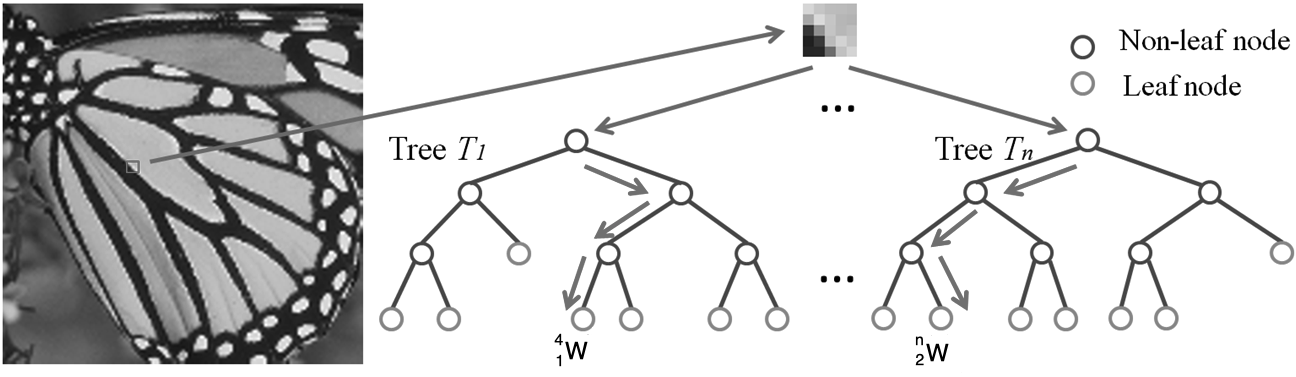
\includegraphics[width=\linewidth,keepaspectratio]{figures/classical/FIRF.png}
    \caption{A set of decision trees. Each decision tree recursively classifies the input LR patch into left or right child node, until a leaf node is reached. By using the linear regression models stored in the each leaf node, the input LR patch can be projected to the HR patch space \cite{Huang}.}
    \label{fig:firf}
\end{figure}
%
Finally the inferred HR patch \(\by\) is the average of patches \(\prescript{l}{t}{\hat{W}(\bx)}\) inferred by all \(n\) trees in the forest:
\begin{equation}
    \hat{\by} = \frac{1}{n} \sum_{t=1}^{n} \prescript{l}{t}{\hat{W}(\bx)} =  \frac{1}{n} \sum_{t=1}^{n} \sum_{i=1}^I \prescript{l}{t}{\hat{w}_i}\phi_i(\bx)
\end{equation}
where \(l = l(t)\) is the leaf that sample \(\bx\) is routed to for each tree \(t\).
%
Schulter \etal train the trees on example LR-HR patch pairs \(\bx, \by\) by recursively splitting the data using parameterized splitting functions
\begin{equation}
    \sigma(\bx, i, j, \tau)\coloneqq {
        \begin{cases}
            \text{left}  & \text{if } \text{vec}(\bx)\left[ i \right] - \text{vec}(\bx)\left[ j \right] - \tau < 0 \\
            \text{right} & \text{otherwise}
        \end{cases}
    }
\end{equation}
where \(\text{vec}(\bx)\left[ i \right]\) is the \(i\)th pixel of \(\text{vec}(\bx)\) and similarly \(\text{vec}(\bx)\left[ j \right]\).
%
The tree is grown as a function of the splitting function, current depth, and current goodness of fit.
%
At each node they select the splitting function parameters \(i, j, \tau\) by evaluating all such possible pixel pairs and thresholds according to a quality measure whose purpose is to cluster similar LR patches:
\begin{equation}
    Q(\bX, \bY) \coloneqq \sum_k \left( \abs{ \by_k - \hat{\by}_k }^2 + \alpha\abs{ \bx_k - \bar{\bx} }^2 \right)
    \label{eqn:qualitymeasure}
\end{equation}
where \(\hat{\by}_k\) is the estimate produced by the linear regression fit using data that's arrived at that node (and \(\alpha\) is a scale regularization parameter).
%
The first term in eqn.~\eqref{eqn:qualitymeasure} measures fitting error and the second term is the clustering regularizer.
%
They decide whether to actually split according to the \textit{error reduction} in performing the split:
\begin{multline*}
    R\left(i, j, \tau, \bX, \bY \right) \coloneqq \\ Q(\bX, \bY) - \sum_{c\in\left\{L, R\right\}} \frac{\abs{\bX^c}}{\abs{\bX}} Q(\bX^c, \bY^c)
\end{multline*}
where \(\bX^L\) are all of the \(\bx_k\) such that \(\sigma(\bx_k, i, j, \tau) = \text{ left }\) and \(\bY^L\) are all the corresponding \(\by_k\) (and similarly for \(\bX^R, \bY^R\)).
%
The best set of parameters \(\hat{\imath}, \hat{\jmath}, \hat{\tau}\) are those that maximize \(R\left(i, j, \tau, \bX, \bY \right)\).
%
Then if \(R\left(\hat{\imath}, \hat{\jmath}, \hat{\tau}, \bX, \bY \right)\) is greater than zero (i.e., there's an error reduction gained from performing the split) the data is split amongst the left child and right child.
%
Each non-leaf node stores its best set of parameters and each leaf node stores its learned linear regression.